\documentclass{article}

\usepackage[margin=.75in]{geometry}
\usepackage{amsmath}
\usepackage{amssymb}
\usepackage[shortlabels]{enumitem}
\usepackage{pgfplots}
\usepackage{circuitikz}
\usepackage{float}
\usepackage{verbatim}

\author{Damien Prieur}
\title{Homework 6\\ ECES 512}
\date{}

\begin{document}

\maketitle

\section*{Problem 1}
Consider a plant described by
$$
\dot{x} =
\begin{bmatrix}
1 & 3 \\
3 & 1 \\
\end{bmatrix}
x
+
\begin{bmatrix}
1 \\
0 \\
\end{bmatrix}
u
$$

\begin{enumerate}[a.]
\item Find out if the system is stable.
\newline
We can look at the eigenvalues of the $A$ matrix as we are only looking at internal stability since the states are the output variables.
$$
det(
\begin{bmatrix}
\lambda & 0 \\
0 & \lambda \\
\end{bmatrix}
-
\begin{bmatrix}
1 & 3 \\
3 & 1 \\
\end{bmatrix}
)=
\begin{vmatrix}
\lambda-1 & -3 \\
-3 & \lambda-1 \\
\end{vmatrix}
=0
$$
$$(\lambda-1)^2 -9 = 0$$
$$(\lambda-1)^2 = 9$$
$$\lambda-1 = \pm 3$$
$$\lambda = 1 \pm 3$$
$$\lambda_1 = -2 \quad \lambda_2 = 4 $$
Since we have eigenvalues on the right half of the plane our system is unstable.

\item Find out if the system is controllable.
\newline
Since the plant is LTI we can use the rank of the controllability matrix $\begin{bmatrix}B & AB\end{bmatrix}$
$$
AB =
\begin{bmatrix}
1 & 3 \\
3 & 1 \\
\end{bmatrix}
\begin{bmatrix}
1 \\
0 \\
\end{bmatrix}
=
\begin{bmatrix}
1 \\
3 \\
\end{bmatrix}
$$
$$
C = \begin{bmatrix}B & AB\end{bmatrix} =
\begin{bmatrix}
1 & 1 \\
0 & 3 \\
\end{bmatrix}
$$
We can see that the rank of the controllability matrix is 2 which is full rank. The system is controllable.

\item Use direct coefficients matching method to find the K that shifts the poles to $-1\pm j2$.
\newline
$$
u = -Kx \qquad
\dot{x}
=
(
\begin{bmatrix}
1 & 3 \\
3 & 1 \\
\end{bmatrix}
-
\begin{bmatrix}
1 \\
0 \\
\end{bmatrix}
\begin{bmatrix} k_1 & k_2 \end{bmatrix}
)
x
$$
$$
\dot{x}
=
(
\begin{bmatrix}
1 & 3 \\
3 & 1 \\
\end{bmatrix}
-
\begin{bmatrix}
k_1 & k_2 \\
0   &  0  \\
\end{bmatrix}
)
x
=
\begin{bmatrix}
1-k_1 & 3-k_2 \\
3 & 1 \\
\end{bmatrix}
x
$$
We want to find the $k$'s that satisfy this equation
$$|sI-(A-BK)| = (s-(-1+j2))(s-(-1-j2))$$
$$
\begin{vmatrix}
s + k_1 -1 & k_2 - 3 \\
-3         & s-1 \\
\end{vmatrix}
= s^2 + 2s + 5
$$
$$
(s + k_1 -1)(s-1)+3(k_2 - 3)
= s^2 + 2s + 5
$$
$$
s^2 + (k_1-2)s -k_1 + 3k_2-8
= s^2 + 2s + 5
$$
Matching Coefficients we get two equations
$$ 2 = k_1-2 \qquad 5 = 3k_2 -k_1-8 $$
Solving for each we get
$$ k_1 = 4 \qquad k_2 = \frac{17}{3} $$

\item Apply Ackermann's formula to find the same K in part c.
\newline
We have the formula
$$ k^T = \begin{bmatrix}0 & 1 \end{bmatrix} \mathcal{C}^{-1} \Delta (A) $$
We have the desired poles as $ \Delta (x) = x^2 + 2x + 5 $
$$ k^T =
\begin{bmatrix} 0 & 1 \end{bmatrix}
\begin{bmatrix}
1 & 1 \\
0 & 3 \\
\end{bmatrix}
^{-1}
(
\begin{bmatrix}
1 & 3 \\
3 & 1 \\
\end{bmatrix}
^2
+
2
\begin{bmatrix}
1 & 3 \\
3 & 1 \\
\end{bmatrix}
+
\begin{bmatrix}
5 & 0 \\
0 & 5 \\
\end{bmatrix}
)
$$
$$ k^T =
\begin{bmatrix} 0 & 1 \end{bmatrix}
\frac{1}{3}
\begin{bmatrix}
3 & -1 \\
0 &  1 \\
\end{bmatrix}
(
\begin{bmatrix}
10 &  6 \\
 6 & 10 \\
\end{bmatrix}
+
\begin{bmatrix}
7 & 6 \\
6 & 7 \\
\end{bmatrix}
)
$$
$$ k^T =
\frac{1}{3}
\begin{bmatrix} 0 & 1 \end{bmatrix}
\begin{bmatrix}
17 & 12 \\
12 & 17 \\
\end{bmatrix}
$$
$$ k^T = \begin{bmatrix} 4 & \frac{17}{4} \end{bmatrix} $$
$$ k_1 = 4 \qquad k_2 = \frac{17}{4} $$

\item Repeat part c and part d in Matlab by using the function $place$ and $acker$.
\newline
\verbatiminput{Homework_6_1.m}

\item Simulate the time domain solution of the system before and after shifting the poles and explain. The input is the unit step function.
\newline
\begin{figure} [H]
    \centering
    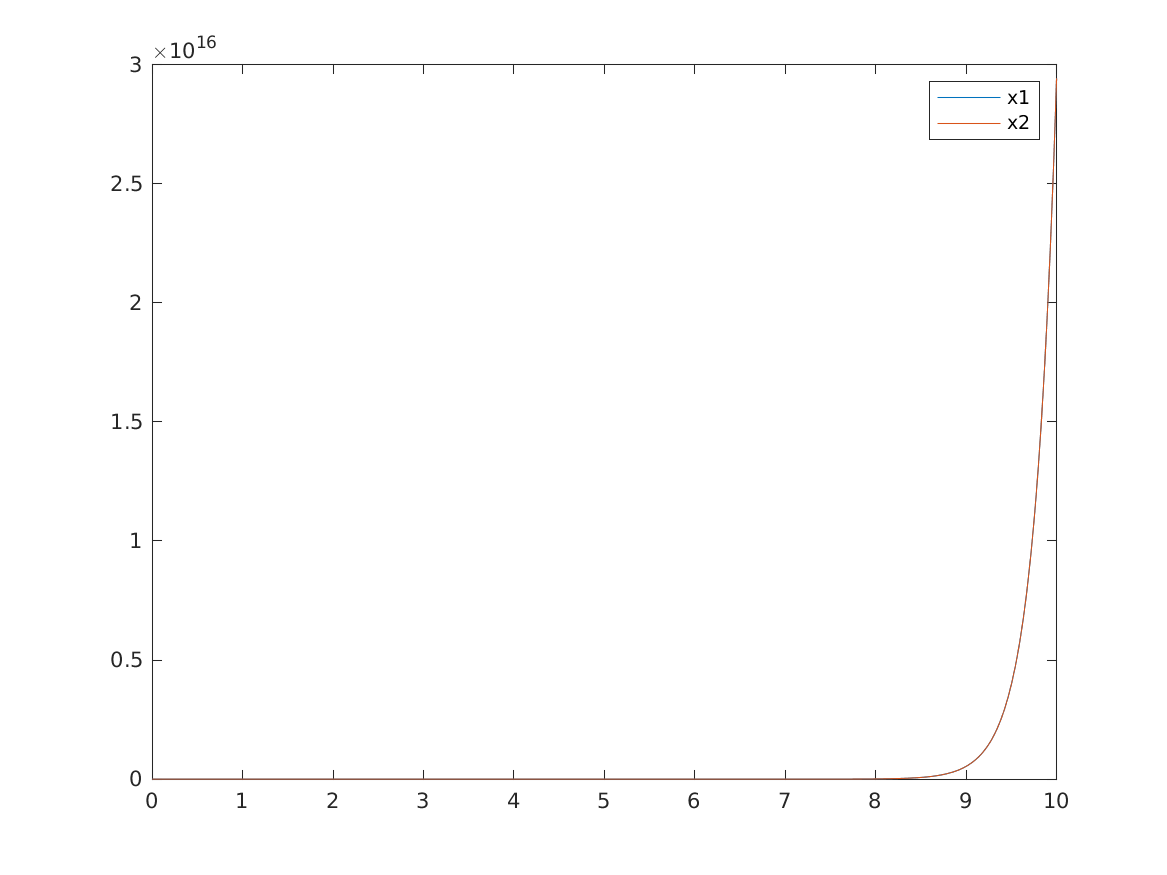
\includegraphics[width=.65\linewidth]{{images/p1_original_system}.png}
    \caption{Original System}
    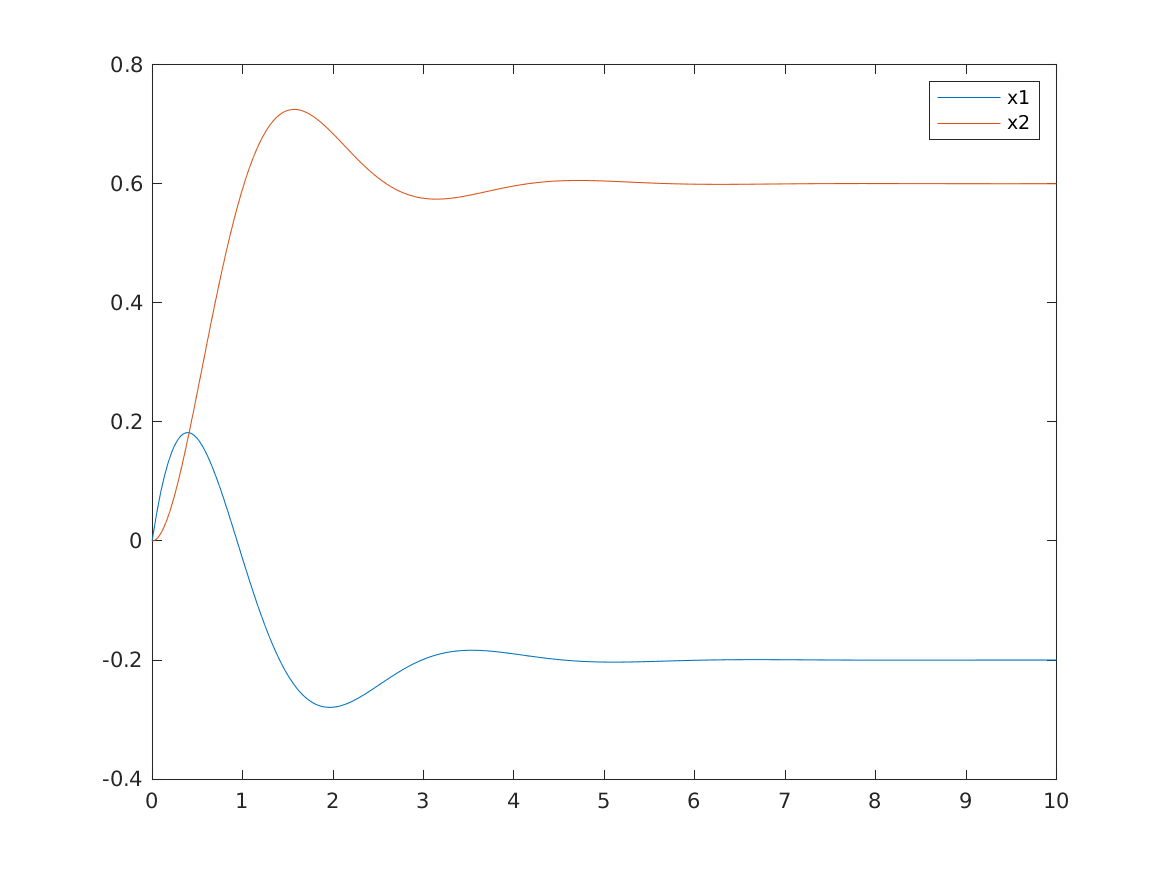
\includegraphics[width=.65\linewidth]{{images/p1_modified_system}.png}
    \caption{Modified System}
\end{figure}
In the original system the system is unstable due to the poles in the right right half plane.
This causes the states to blow up towards infinity, but once we move the poles the system is no longer unstable.
We can see that the system stabilized now that the poles are in the left half plane.
The oscillation in the transient can be explained by the complex components of the poles which eventually get dampened out.

\end{enumerate}

\newpage
\section*{Problem 2}

Consider a plant described by

$$
\dot{x} =
\begin{bmatrix}
1 & 1 & -2 \\
0 & 1 &  1 \\
0 & 0 &  1 \\
\end{bmatrix}
x
+
\begin{bmatrix}
1 \\
0 \\
1 \\
\end{bmatrix}
u
\qquad
y = \begin{bmatrix} 2 & 0 & 0 \end{bmatrix} x 
$$

\begin{enumerate}[a.]
\item Find out if the system is stable.
\newline
We can check for internal stability by looking at the eigenvalues and check for BIBO stability by looking at the transfer function.
\newline
Since the $A$ matrix is upperdiagonal the eigenvalues are already on the diagonal.
We can see that we have 3 repeated eigenvalues of $1$
$$ \lambda_1 = \lambda_2 = \lambda_3 = 1 $$
For BIBO stability we look at
$$
C|sI-A|^{-1}B =
\begin{bmatrix} 2 & 0 & 0 \end{bmatrix}
(
\begin{bmatrix}
s & 0 & 0 \\
0 & s & 0 \\
0 & 0 & s \\
\end{bmatrix}
-
\begin{bmatrix}
1 & 1 & -2 \\
0 & 1 &  1 \\
0 & 0 &  1 \\
\end{bmatrix}
)^{-1}
\begin{bmatrix}
1 \\
0 \\
1 \\
\end{bmatrix}
$$
$$
\begin{bmatrix} 2 & 0 & 0 \end{bmatrix}
\begin{bmatrix}
s-1 & -1 & 2 \\
0 & s-1 &  -1 \\
0 & 0 &  s-1 \\
\end{bmatrix}
^{-1}
\begin{bmatrix}
1 \\
0 \\
1 \\
\end{bmatrix}
$$
We can find the inverse of the Matrix more easily since it is upper triangular using the formula
$$
\begin{bmatrix}
a & b & c \\
0 & d & e \\
0 & 0 & f \\
\end{bmatrix}
^{-1}
=
\begin{bmatrix}
\frac{1}{a} & \frac{-b}{ad} & \frac{be-cd}{adf} \\
0 & \frac{1}{d} & \frac{-e}{df} \\
0 & 0 & \frac{1}{f} \\
\end{bmatrix}
$$
Plugging in we get
$$
\begin{bmatrix} 2 & 0 & 0 \end{bmatrix}
\begin{bmatrix}
\frac{1}{s-1} & \frac{1}{(s-1)^2} & \frac{3-2 s}{(s-1)^3} \\
0 & \frac{1}{s-1} & \frac{1}{(s-1)^2} \\
0 & 0 & \frac{1}{s-1} \\
\end{bmatrix}
\begin{bmatrix}
1 \\
0 \\
1 \\
\end{bmatrix}
$$
$$
\begin{bmatrix}
\frac{2}{s-1} & 0 & 0
\end{bmatrix}
\begin{bmatrix}
1 \\
0 \\
1 \\
\end{bmatrix}
$$
$$\frac{2}{s-1}$$
Which only has a single pole in the right half plane.
Therefore the system is not BIBO stable.

\item Find out if the system is controllable.
\newline
Since the plant is LTI we can use the rank of the controllability matrix $\begin{bmatrix}B & AB & A^2B\end{bmatrix}$
$$
AB =
\begin{bmatrix}
1 & 1 & -2 \\
0 & 1 &  1 \\
0 & 0 &  1 \\
\end{bmatrix}
\begin{bmatrix}
1 \\
0 \\
1 \\
\end{bmatrix}
=
\begin{bmatrix}
-1 \\
 1 \\
 1 \\
\end{bmatrix}
$$
$$
A^2B =
\begin{bmatrix}
1 & 1 & -2 \\
0 & 1 &  1 \\
0 & 0 &  1 \\
\end{bmatrix}
^2
\begin{bmatrix}
1 \\
0 \\
1 \\
\end{bmatrix}
=
\begin{bmatrix}
1 & 2 & -3 \\
0 & 1 & 2 \\
0 & 0 & 1 \\
\end{bmatrix}
\begin{bmatrix}
1 \\
0 \\
1 \\
\end{bmatrix}
=
\begin{bmatrix}
-2 \\
2 \\
1 \\
\end{bmatrix}
$$
$$
C = \begin{bmatrix}B & AB & A^2B\end{bmatrix} =
\begin{bmatrix}
1 & -1 & -2 \\
0 & 1 & 2   \\
1 & 1 & 1   \\
\end{bmatrix}
$$
By performing the two row operations of subtracting the first two rows from the last row we get
$$
\begin{bmatrix}
1 & -1 & -2 \\
0 & 1 & 2   \\
0 & 0 & -1  \\
\end{bmatrix}
$$
We can see that the rank of the controllability matrix is 3 which is full rank. The system is controllable.

\item Use direct coefficients matching method to find the K so that the resulting system has eigenvalues -2 and $-1\pm j1$.
\newline
$$
u = -Kx \qquad
\dot{x}
=
(
\begin{bmatrix}
1 & 1 & -2 \\
0 & 1 &  1 \\
0 & 0 &  1 \\
\end{bmatrix}
-
\begin{bmatrix}
1 \\
0 \\
1 \\
\end{bmatrix}
\begin{bmatrix} k_1 & k_2 & k_3 \end{bmatrix}
)
x
$$
$$
\dot{x}
=
(
\begin{bmatrix}
1 & 1 & -2 \\
0 & 1 &  1 \\
0 & 0 &  1 \\
\end{bmatrix}
-
\begin{bmatrix}
k_1 & k_2 & k_3 \\
0 & 0 &  0 \\
k_1 & k_2 & k_3 \\
\end{bmatrix}
)
x
=
\begin{bmatrix}
1-k_1 & 1-k_2 & -2-k_3 \\
0 & 1 &  1 \\
-k_1 & -k_2 &  1-k_3 \\
\end{bmatrix}
x
$$
We want to find the $k$'s that satisfy this equation
$$|sI-(A-BK)| = (s+2)(s-(-1+j))(s-(-1-j))$$
$$
\begin{vmatrix}
s+k_1-1 & k_2-1 & k_3+2 \\
0 & s-1 &  -1 \\
k_1 & k_2 &  s+k_3-1 \\
\end{vmatrix}
= s^3 + 4 s^2 +6 s + 4
$$
$$
(s + k_1 -1)(s-1)(s+k_3-1)k_2 + k_1(1-k_2)(k_3+2)(1-s)
= s^3 + 4 s^2 +6 s + 4
$$
$$
s^3 + (k_1 + k_3 -3) s^2 + (-4 k_1 + k_2 - 2k_3 + 3) s + (4k_1 -k_2 + k_3 - 1)
= s^3 + 4 s^2 +6 s + 4
$$
Matching Coefficients we get three equations
$$ k_1 + k_3 -3 = 4 \qquad  -4 k_1 + k_2 - 2k_3 + 3 = 6 \qquad 4k_1 -k_2 + k_3 - 1 = 4 $$
We can rewrite this into matrix form for easier solving
$$
\begin{bmatrix}
1 & 0 & 1 \\
-4 & 1 & -2 \\
4 & -1 & 1\\
\end{bmatrix}
\begin{bmatrix}
k_1\\
k_2\\
k_3\\
\end{bmatrix}
=
\begin{bmatrix}
7\\
3\\
5\\
\end{bmatrix}
$$
Solving for each we get
$$ k_1 = 15 \qquad k_2 = 47 \qquad k_3 = -8 $$

\item Apply Ackermann's formula to find the same K in part c.
\newline
We have the formula
$$ k^T = \begin{bmatrix}0 & 0 & 1 \end{bmatrix} \mathcal{C}^{-1} \Delta (A) $$
We have the desired poles as $ \Delta (x) = x^3 + 4x^2 + 6x + 4 $
$$ k^T =
\begin{bmatrix} 0 & 0 & 1 \end{bmatrix}
\begin{bmatrix}
1 & -1 & -2 \\
0 & 1 & 2   \\
0 & 0 & -1  \\
\end{bmatrix}
^{-1}
(
\begin{bmatrix}
1 & 1 & -2 \\
0 & 1 &  1 \\
0 & 0 &  1 \\
\end{bmatrix}
^3
+
4
\begin{bmatrix}
1 & 1 & -2 \\
0 & 1 &  1 \\
0 & 0 &  1 \\
\end{bmatrix}
^2
+
6
\begin{bmatrix}
1 & 1 & -2 \\
0 & 1 &  1 \\
0 & 0 &  1 \\
\end{bmatrix}
+
\begin{bmatrix}
4 & 0 & 0 \\
0 & 4 & 0 \\
0 & 0 & 4 \\
\end{bmatrix}
)
$$
From part A we have a closed form solution to the matrix inverse since we are upper diagonal.
$$ k^T =
\begin{bmatrix} 0 & 0 & 1 \end{bmatrix}
\begin{bmatrix}
 1 &  1 &  0  \\
-2 & -3 & -2  \\
 1 &  2 & -1  \\
\end{bmatrix}
(
\begin{bmatrix}
1 & 3 & -3 \\
0 & 1 &  3 \\
0 & 0 &  1 \\
\end{bmatrix}
+
4
\begin{bmatrix}
1 & 2 & -3 \\
0 & 1 &  2 \\
0 & 0 &  1 \\
\end{bmatrix}
+
\begin{bmatrix}
10 & 6 & -12 \\
0 & 10 & 6 \\
0 & 0 & 10 \\
\end{bmatrix}
)
$$
$$ k^T =
\begin{bmatrix} 0 & 0 & 1 \end{bmatrix}
\begin{bmatrix}
 1 &  1 &  0  \\
-2 & -3 & -2  \\
 1 &  2 & -1  \\
\end{bmatrix}
\begin{bmatrix}
15 & 17 & -27 \\
 0 & 15 &  17 \\
 0 &  0 &  15 \\
\end{bmatrix}
$$
$$ k^T =
\begin{bmatrix} 0 & 0 & 1 \end{bmatrix}
\begin{bmatrix}
 15 &  32 & -10 \\
-30 & -79 &  47 \\
 15 &  47 &  -8 \\
\end{bmatrix}
$$
$$ k^T = \begin{bmatrix} 15 &  47 &  -8 \\ \end{bmatrix} $$
$$ k_1 = 15 \qquad k_2 = 47 \qquad k_3 = -8 $$

\item Repeat part c and part d in Matlab by using the function $place$ and $acker$.
\newline
\verbatiminput{Homework_6_2.m}

\item Simulate the time domain solution of the system before and after shifting the poles and explain. The input is the unit step function.
\newline
\begin{figure} [H]
    \centering
    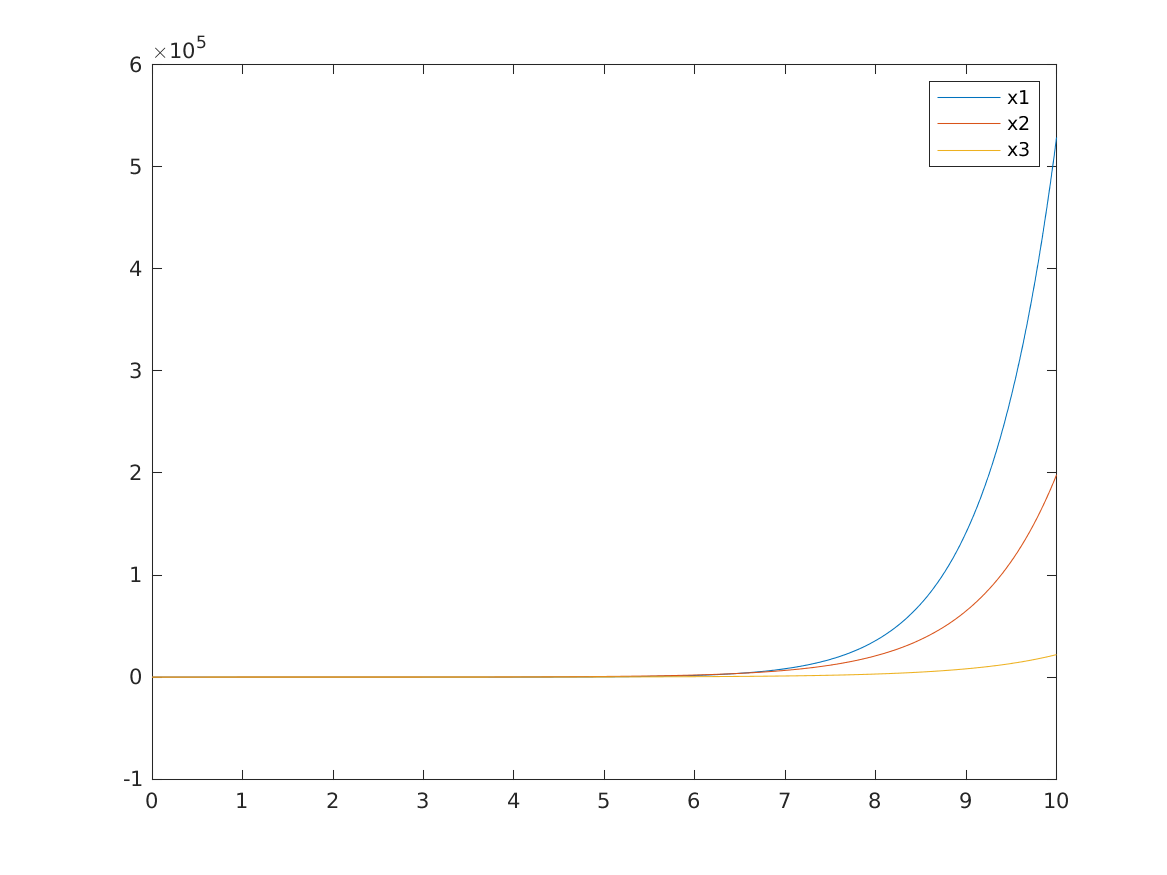
\includegraphics[width=.65\linewidth]{{images/p2_original_system}.png}
    \caption{Original System}
    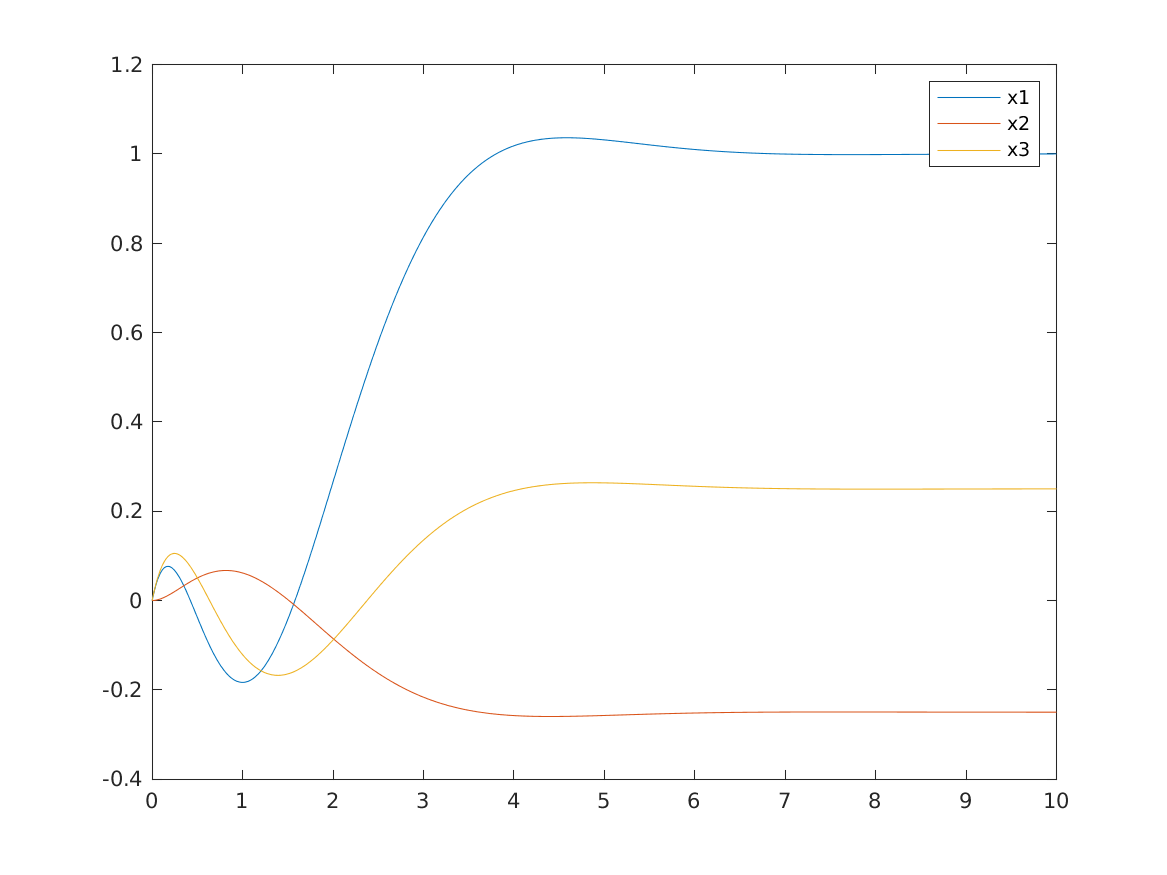
\includegraphics[width=.65\linewidth]{{images/p2_modified_system}.png}
    \caption{Modified System}
\end{figure}
In the original system the system is unstable due to the poles in the right right half plane.
This causes the states to blow up towards infinity, but once we move the poles the system is no longer unstable.
We can see that the system stabilized now that the poles are in the left half plane.
The oscillation in the transient can be explained by the complex components of the poles which eventually get dampened out.

\end{enumerate}

\end{document}
